%%%%%%%%%%%%%%%%%%%%%%%%%%%%%%%%%%%%%%%%%
% University/School Laboratory Report
% LaTeX Template
% Version 3.0 (4/2/13)
%
% This template has been downloaded from:
% http://www.LaTeXTemplates.com
%
% Original author:
% Linux and Unix Users Group at Virginia Tech Wiki 
% (https://vtluug.org/wiki/Example_LaTeX_chem_lab_report)
%
% License:
% CC BY-NC-SA 3.0 (http://creativecommons.org/licenses/by-nc-sa/3.0/)
%
%%%%%%%%%%%%%%%%%%%%%%%%%%%%%%%%%%%%%%%%%

%----------------------------------------------------------------------------------------
%	PACKAGES AND DOCUMENT CONFIGURATIONS
%----------------------------------------------------------------------------------------

\documentclass{article}

\usepackage{mhchem} % Package for chemical equation typesetting
\usepackage{siunitx} % Provides the \SI{}{} command for typesetting SI units
\usepackage[margin=1in]{geometry}
\usepackage{graphicx} % Required for the inclusion of images
\usepackage{pict2e}

\setlength\parindent{0pt} % Removes all indentation from paragraphs

\renewcommand{\labelenumi}{\alph{enumi}.} % Make numbering in the enumerate environment by letter rather than number (e.g. section 6)

%\usepackage{times} % Uncomment to use the Times New Roman font

%----------------------------------------------------------------------------------------
%	DOCUMENT INFORMATION
%----------------------------------------------------------------------------------------

\title{A first look at the energy spectra from the neutron generator in 2D} % Title

\author{Brian Lenardo} % Author name

\date{\today} % Date for the report

\begin{document}

\maketitle % Insert the title, author and date

% If you wish to include an abstract, uncomment the lines below
% \begin{abstract}
% Abstract text
% \end{abstract}

%----------------------------------------------------------------------------------------
%	SECTION 1
%----------------------------------------------------------------------------------------

\section{A rough introduction}
We hope to study the use of a compact, monoenergetic neutron generator to measure ionization and scintillation yields. This will be accomplished using single neutron scatters. To establish the effectiveness of the compact neutron generator, we need to convolve the following details:
\begin{enumerate}
\item Energy spectrum due to the fraction of neutrons that escape after a single scatter for a given angle relative to the radial
\item Attenuation in single scatters due to initial distance through the xenon
\item Error in the position reconstruction
\item Other stuff?
\end{enumerate}

In the following two sections, we study the first item in the list above. To begin, we'll explain the geometrical arguments for the first of the above. We then calculate the expected spectra due to the geometry of the interactions, assuming that the recoils are inherently uniform in energy.

\section{Geometry of the problem}

\begin{figure}
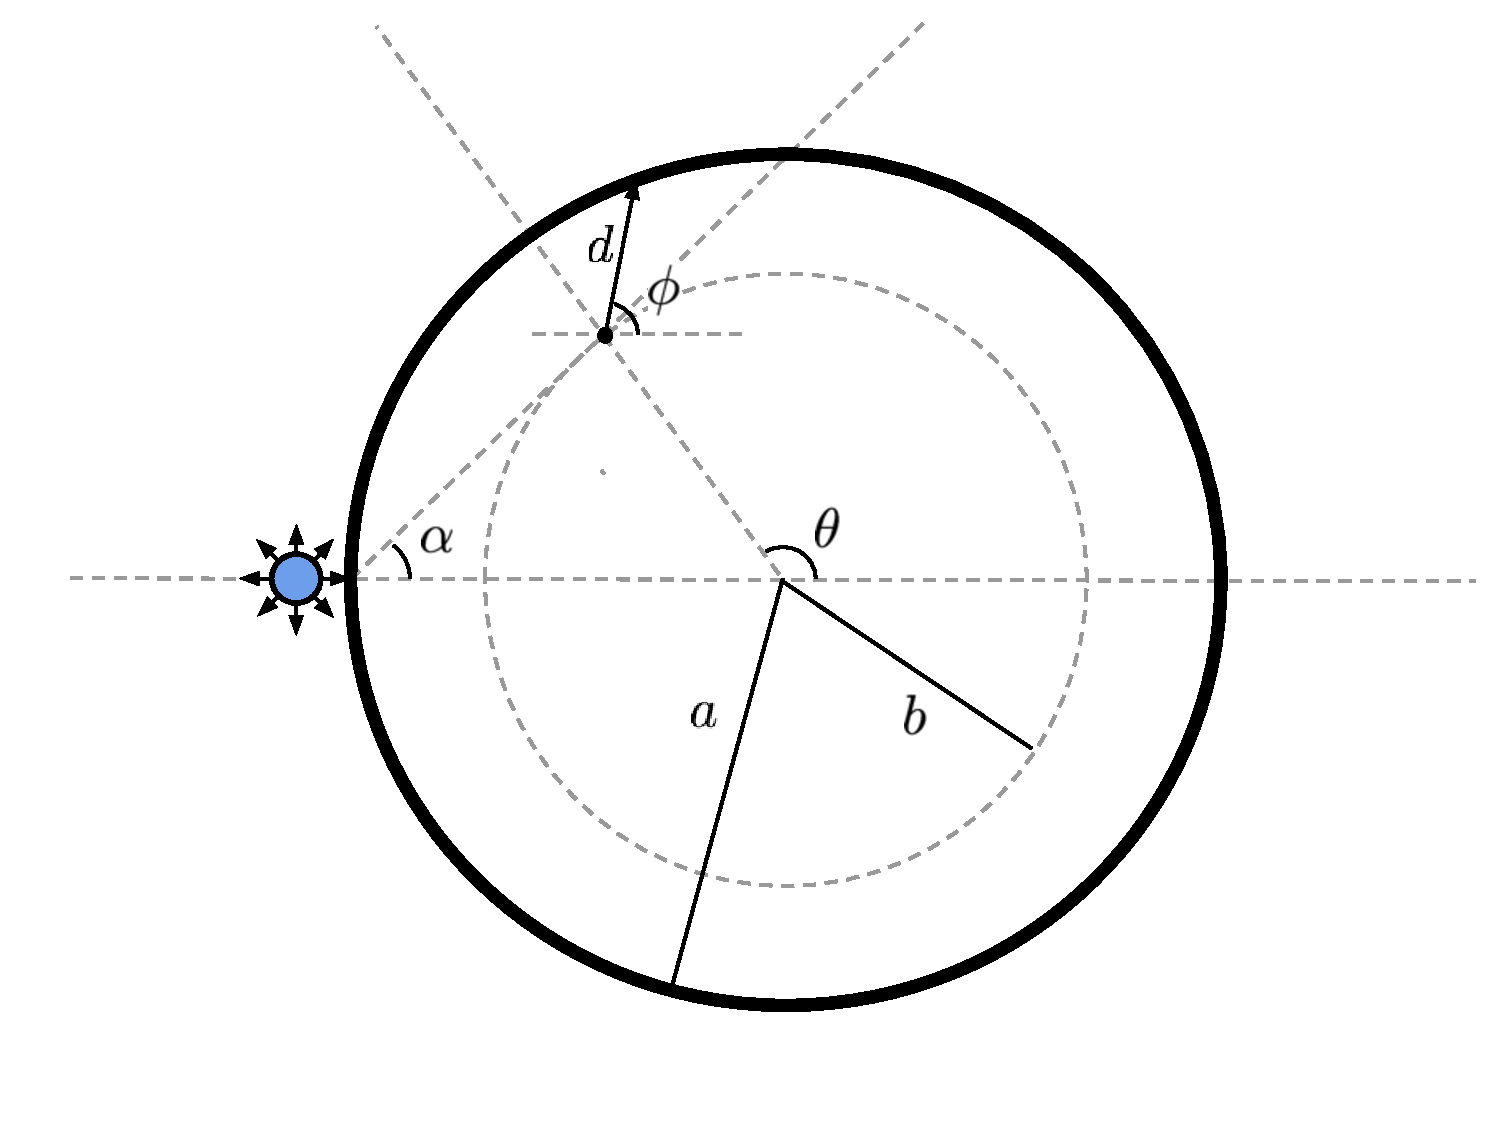
\includegraphics[width=0.8\textwidth]{ProblemCoordinates.pdf}
\centering
\caption{Schematic of the compact neutron generator set-up.}
\end{figure}
We must first find the distance traveled after the single scatter as a function of $a$, $b$, $\theta$, and $\phi$:
\[ d = d(a,b,\theta,\phi) \]
  In order to do so, we'll begin with the cartesian equation for a circle of radius $R$ centered at an arbitrary point $(x_0,y_0)$:
  \[ (x - x_0)^2 + (y - y_0)^2 = R^2\]
 Plugging in for polar coordinates, this becomes:
 \begin{align*}
 (r \,\,\text{cos} \, \beta - x_0)^2 + (r \,\, \text{sin} \, \beta - y_0)^2 &= R^2  \\
r^2 (\text{cos}^2 \, \beta + \text{sin}^2 \, \beta) - 2( x_0 \, \text{cos} \, \beta + y_0 \, \text{sin} \, \beta) \, r + (x_0^2 + y_0^2 - R^2) &= 0 \\
r^2 - 2( x_0 \, \text{cos} \, \beta + y_0 \, \text{sin} \, \beta) \, r + (x_0^2 + y_0^2 - R^2) & = 0
\end{align*}

We can then use the quadratic formula to solve for $r$ as a function of $\beta$:
\[ r = \frac{ ( 2 x_0 \, \text{cos} \, \beta + 2 y_0 \, \text{sin} \, \beta) \pm \sqrt{ ( 2 x_0 \, \text{cos} \, \beta + 2 y_0  \,\text{sin} \, \beta)^2 - 4 \, (x_0^2 + y_0^2 - R^2)  }} {2}  \]
Then, the problem of finding $d(a,b,\theta,\phi)$ amounts to plugging in the correct dimensions for the problem at hand. If we treat the point of the interaction as the origin, we can put the center of the circle at $(x_0,y_0) = (a -b, 0)$.  If this is the case, $\beta = \phi + \pi - \theta$. Then we have:
\[ d(a,b,\theta,\phi) =  b \, \text{cos} \, (\phi + \pi - \theta) \pm \sqrt{  b^2 \, \text{cos}^2 \,(\phi + \pi - \theta)  - \, (b^2 - 2 ab)  } \]
Consulting Fig. 1, we see that in all cases 
\begin{align*}
 & 2ab > b^2 \,\,\,\,\,\,   \\
 & \Longrightarrow \,\,\,\,\,\, \sqrt{ b^2 \, \text{cos}^2 \, (\phi + \pi - \theta) + (2ab - b^2) } > b \, \text{cos} \, (\phi + \pi - \theta)
  \end{align*}
  Because the distance can't be negative by choice of coordinates, we choose the plus sign in the above expression. 
  
\section{Energy distribution}
Now that we have an expression for the length across which attenuation of the signal can occur, we can translate this into an energy spectrum. We assume that the outgoing spectrum is flat, so that, for some constant incoming flux, the number of particles scattered with energy between $E$ and $E + dE$ is given by
\[ \frac{dN}{dE} dE = \frac{N_0}{74 \text{keV}} \, dE   \]
However, in order to find the number of single scatters that we can possibly measure, we must attenuate this signal by a factor of $e\,^{ -d / \lambda}$, where $d$ is the distance the scattered neutron must travel to escape the detector and $\lambda$ is the mean free path of the neutron in liquid xenon. This accounts for the probability that the neutron will scatter a second time and therefore not be a part of our signal. In this case, the number of detectable single scatters is:
\[ \frac{dN}{dE} dE = \frac{N_0}{74 \text{keV}} \, \, e \,^{ -d(E) / \lambda } \, dE \]
We must, using the expression found above for $d(\phi)$, find $d(E)$.  So we need $\phi(E)$.

\subsection{Finding $\phi(E)$}
In the lab frame of reference, the energy is related to the outgoing angle $\Theta$  by:
\[ E_{nr} = E_n \, \frac{4 \, m_n \, m_{Xe}}{(m_n + m_{Xe})^2} \frac{1 - \text{cos} \, \Theta}{2} \]
Referring to Figure 1, we see that $\Theta = \phi - \alpha$, so we must solve for $\alpha$.  Using an analogous procedure to Section 1, we find that 
\[ \alpha = \text{cos}^{-1} \left( \frac{a + b \, \text{cos} \, \theta}{\sqrt{a^2 + b^2 + 2 a b \, \text{cos} \, \theta}} \right) \]
\, \\ \, \\
So the nuclear recoil energy can be expressed in terms of $a$, $b$, $\theta$, and $\phi$:
\[ E_{nr} = E_n \, \frac{2 \, m_n \, m_{Xe}}{(m_n + m_{Xe})^2} \left[1 - \text{cos} \, \left( \phi - \text{cos}^{-1} \left( \frac{a + b \, \text{cos} \, \theta}{\sqrt{a^2 + b^2 + 2 a b \, \text{cos} \, \theta}} \right) \, \right)  \right] \]
Letting $ \displaystyle M = \left( E_n \, \frac{2 \, m_n \, m_{Xe}}{(m_n + m_{Xe})^2} \right) $ and solving for $\phi$ gives
\[ \phi (E) = \, \text{cos}^{-1} \, \left( 1 - \frac{E_{nr}}{M} \right) + \alpha \]
  
\subsection{Putting it all together}
When we put all of these pieces together, we find
\begin{align*}
&\frac{dN}{dE} dE = \frac{N_0}{74 \text{keV}} \, \, \\
& \times \exp \left( - \frac{ b \, \text{cos} \, (\text{cos}^{-1} \, \left( 1 - \frac{E_{nr}}{M} \right) + \alpha + \pi - \theta) + \sqrt{  b^2 \, \text{cos}^2 \,(\text{cos}^{-1} \, \left( 1 - \frac{E_{nr}}{M} \right) + \alpha + \pi - \theta)  - \, (b^2 - 2 ab)  }  } {\lambda } \right)  \, dE
 \end{align*}
 
 
This formula allows us to calculate the spectrum that we expect to see when we look at single scatters at a specific point inside the detector.  Example spectra are shown in Figure 2. Here, we assume the detector has radius $a = 25$ cm, and the points of interaction $I_{1-5}$ have radii $b = 20$ cm and various angles $\theta$. 
\begin{figure}
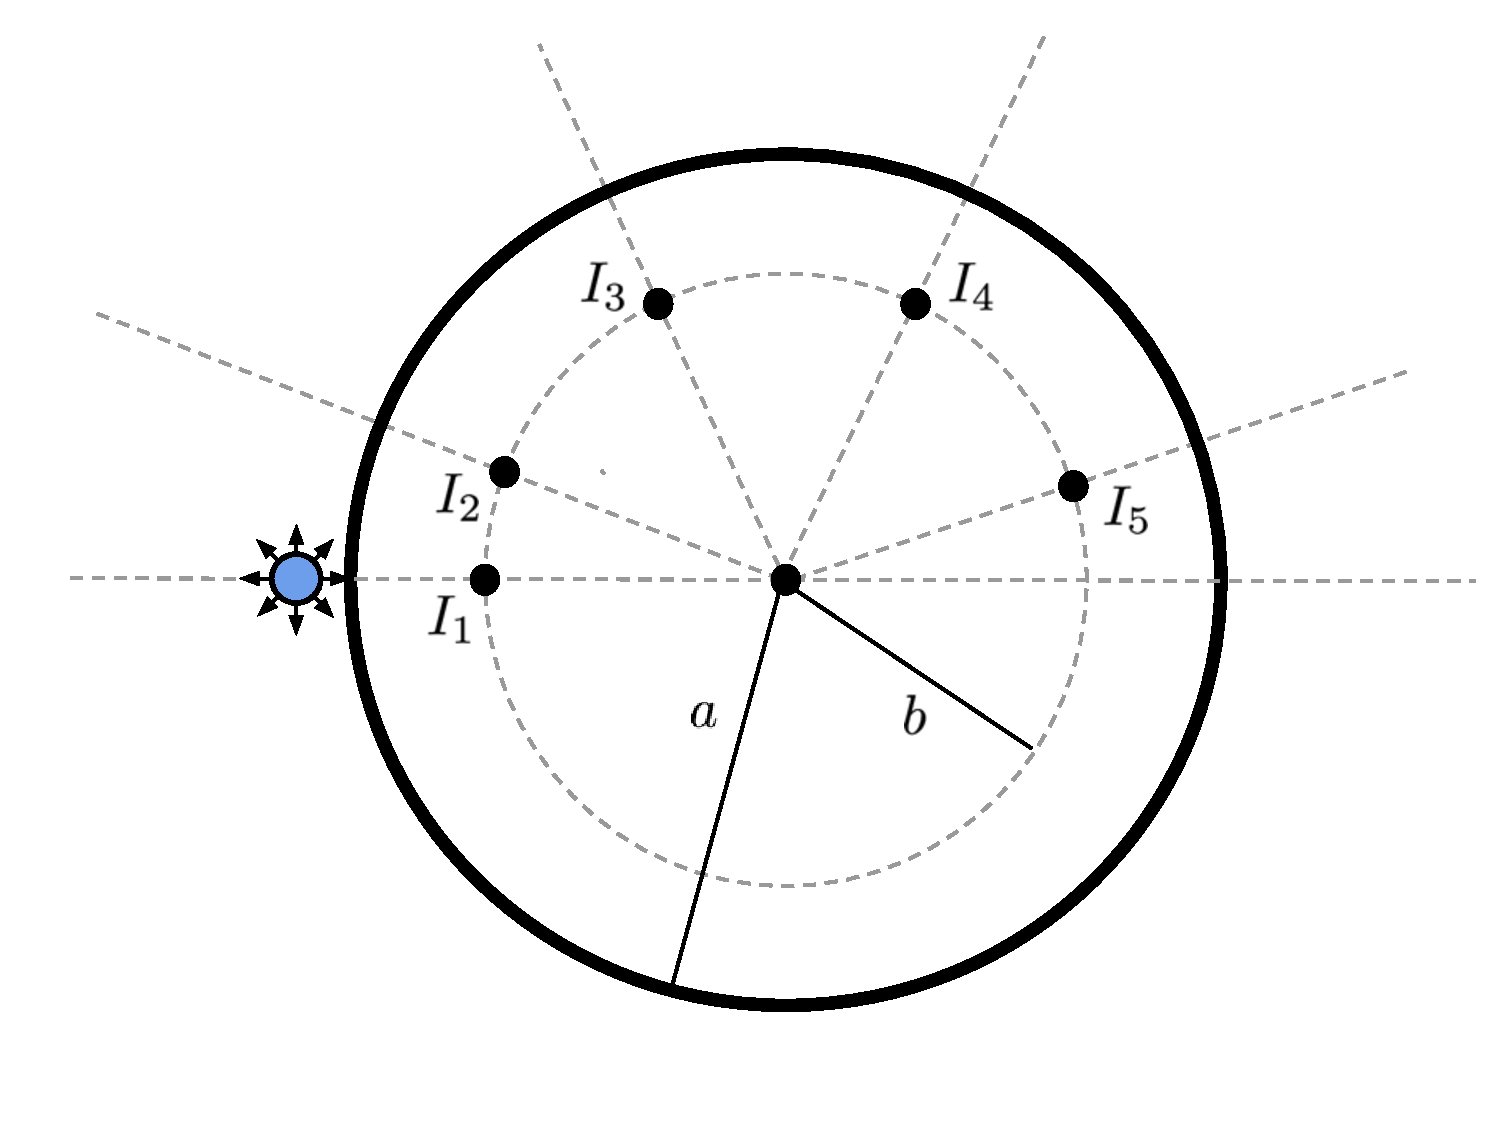
\includegraphics[width=0.8\textwidth]{Points.pdf}
\centering
\caption{Points at which spectra were calculated. They are at $\theta$ = $\pi$, $7 \, \pi / 8$, $5 \, \pi / 8$, $3 \, \pi / 8$, and $\pi / 8$ }
\end{figure}

\begin{figure}
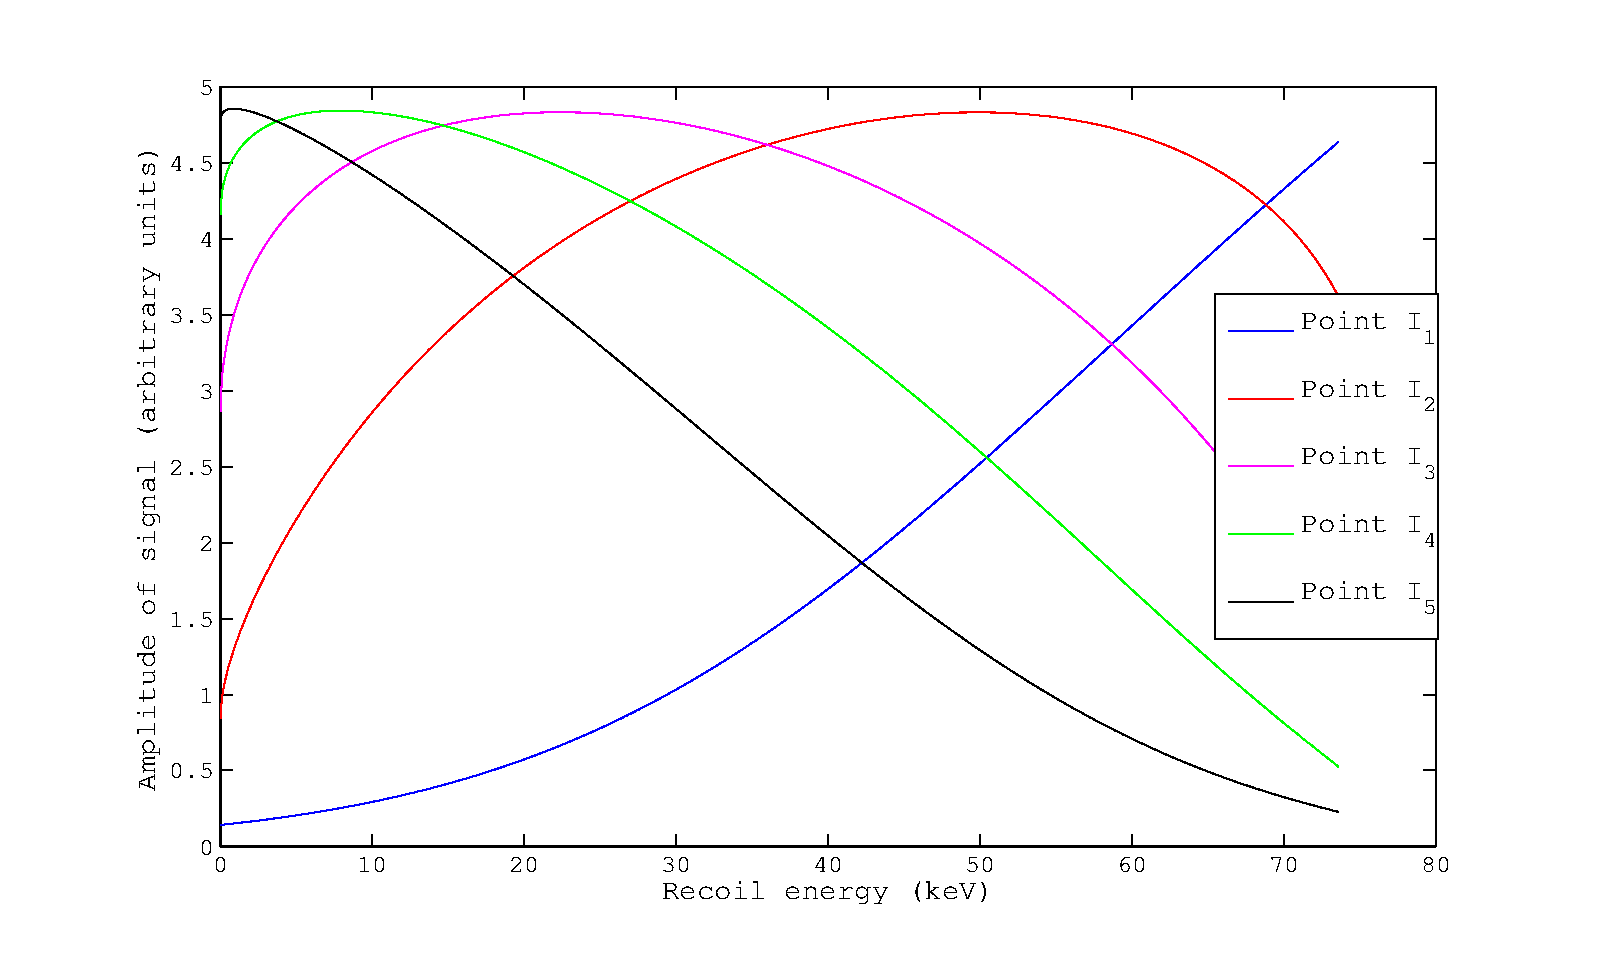
\includegraphics[width=0.8\textwidth]{SpectraAtDifferentAngles.eps}
\centering
\caption{Energy spectra at different points inside the detector, not normalized for initial attenuation.}

\end{figure}




% If you have more than one objective, uncomment the below:
%\begin{description}
%\item[First Objective] \hfill \\
%Objective 1 text
%\item[Second Objective] \hfill \\
%Objective 2 text
%\end{description}


%----------------------------------------------------------------------------------------
%	BIBLIOGRAPHY
%----------------------------------------------------------------------------------------

\bibliographystyle{unsrt}

\bibliography{sample}

%----------------------------------------------------------------------------------------


\end{document}
